\documentclass[a4paper,11pt]{report}
\usepackage{a4wide}
\usepackage[frenchb]{babel}
\usepackage[utf8]{inputenc}
\usepackage[T1]{fontenc}
\usepackage{geometry}
\usepackage{graphicx}
\usepackage{fancybox}
\usepackage[pdftex]{hyperref} %Liens dans table de matieres
\usepackage{fancyhdr}
\usepackage{geometry}
\usepackage{url}
\usepackage{multicol}

\usepackage{pstricks}

%\geometry{scale=0.75, nohead}


\newcommand*{\enConstruction}[1]{
	\vspace*{.1cm}
	\doublebox{
	    \begin{minipage}{.9\linewidth}
	      --- #1 \\ 
	    \end{minipage}
	}
}

\newcommand*{\precision}[1]{
	\vspace*{.1cm}
	\fbox{
		\begin{minipage}{.9\linewidth}
			#1 
		\end{minipage}
  	}\\
}

% Title Page
\title{
	
\includegraphics[scale=.2]{logofds.eps}\\
	\vspace*{1cm}
	TER FMIN200 \\ 
	-- \\
	Développement d'un jeu de type Bomberman en réseau sous Android et iOS
}

\author{BONVILA Olivier \and COUSEIN Kilian \and PITIOT Ludovic \and TARDIEU Benjamin}

\date{}

\begin{document}
\maketitle

\thanks{

  Nous tenons à remercier 

}


\tableofcontents

\chapter{Introduction}

	Nous sommes amenés, dans le cadre de notre première année en master informatique à la faculté des Sciences de Montpellier, à travailler sur l’élaboration complète d’un projet, de son analyse à la conception puis à sa programmation. Tout au long de ce deuxième semestre, le projet nous permet de comprendre quelles sont les phases de développement d’un projet et comment celui-ci doit être conduit. Nous pouvons par ailleurs mesurer notre capacité à réagir face à des problèmes en nous impliquant dans ce projet. Le projet que nous avons choisi constiste à réaliser sur deux \glspl{os} de téléphone différents un jeu de type Bomberman.

Ce projet nous permet de mettre en application l'enseignement que nous avons acquis tout au long de ce semestre. Ce dernier étant spécialisé pour chaque étudiant, il nous a permis de travailler en collaboration avec des personnes aux capacités différentes et d'ainsi mettre nos connaissances en commun. Mais il permet aussi de se faire une idée du travail demandé dans le monde des entreprises et d'ainsi nous préparer à notre stage que nous devrons réaliser l'an prochain.

Afin de comprendre la démarche que nous avons utilisée pour mener ce projet à son terme, notre rapport se compose de cinq grandes parties : 

Tout d'abord, dans une première partie, nous présentons le cadre général de notre projet ainsi que le jeu que nous avons développé. Ensuite, dans une seconde, partie nous verrons comment nous nous sommes orgnanisé pour mener à bien la conduite de notre projet. Puis dans une troisième partie, nous présenterons le travail d'analyse que nous avons effectué pour pouvoir ensuite, dans une quatrième partie, expliquer le developpement du projet. Enfin, nous finirons en expliquant l'implémentation de la réutilisabilité dans le code pour pouvoir ensuite finir sur la conclusion.

\chapter{Présentation}

	\begin{itemize}
		\item{Nous + Tuteur}
	\end{itemize}

	En tant que première année de master, nous avons dû developper un projet tout au long de ce semestre. Chaque année une liste de projets est présentée aux étudiants. Tous les étudiants doivent former des groupes pour développer l'un des projets choisi. Puis ces derniers sont associés à un tuteur. Etant donné que nous voulions développer notre propre projet, nous avons formé un groupe de quatre personnes : Olivier BONVILA, Kilian COUSEIN, Ludovic PITIOT et Benjamin TARDIEU. Ensuite, pour pouvoir valider notre sujet, nous avons dû trouver un tuteur voulant bien s'occuper de notre tutelle. Mr Laurent Deruelle a gentiment accepté de s'occuper de notre groupe, mais pour que ce dernier soit entièrement validé, des modifications du sujet ont été nécessaires.

\section{Projet}	
	
 Etant donné que nous voulions principalement créer une application
 \gls{iphone}, nous avons demandé à développer notre propre projet. Un jeu de
 type Bomberman. Mais ce dernier a dû subir des modifications pour être
 approuvé. Nous avons donc dû développer le jeu sous \gls{iphone} et sous
 \gls{android}. Le but étant de comparer la différence de développement entre
 les deux types de téléphones et de développer des fonctionnalités en rapport
 avec les parcours d'enseignement que nous avons choisi ce semestre.\\
	
	
Pour pouvoir rapprocher le développement de cette application à notre parcours
d'enseignement. Nous avons choisi de développer un mode solitaire qui permettra
de jouer contre une ou plusieurs intelligences artificelles qui est en rapport
avec le cursus \gls{i2a} qui nous est enseigné. Ensuite, pour ce qui est du
parcours \gls{casar}, nous avons décidé d'implémenter un mode multijoueur qui
permettra à plusieurs joueurs connectés en \gls{wi-fi} de jouer en réseau grâce
à un serveur qui combinera un serveur d'applications et un serveur web. Pour ce qui est de la conception de toute la structure du programme nous avons mis en application nos connaissances apprises dans le parcours \gls{gl}. Puis pour ce qui est du parcours \gls{diweb}, la partie serveur permettra de palier à
l'enseignement de ce dernier. 
	


\section{Plate-formes de développement}
	\subsection{Android}
	\begin{itemize}
		\item{De qui ?}
		\item{Langage}
		\item{PC}
		\item{SDK - (le contenu)}
	\end{itemize}

\subsection{iOS}
	\begin{itemize}
		\item{De qui ?}
		\item{Langage}
		\item{Mac}
		\item{SDK - (le contenu)}
	\end{itemize}
	
\section{Organisation}
			Les gestionnaires de versions comme leur nom l'indique, permettent d'avoir à
		porté de main toutes les versions qu'il y a eu d'un fichier depuis sa
		création, cela permet donc de pouvoir revenir en arrière si une erreur a été commise.
		De plus grâce à cela, notre projet reste cohérent dans le sens où pour pouvoir
		être mis à jour, il faut à tout prit avoir modifié un fichier à partir de la
		dernière version de celui-ci.
		
		Dernier avantage d'avoir utilisé un gestionnaire de version et qu'il est
		hébérgé sur le net et donc chaque membre de l'équipe peut y accéder où qu'il
		soit. 
		
		De plus \emph{\gls{google_code}} met aussi à disposition de ses utilisateurs des \glspl{wiki}.
		Un \gls{wiki} est un site Web dont les pages sont modifiables par les développeurs
		afin de permettre l'écriture et l'illustration collaboratives des documents numériques qu'il contient.
		
		Malgré de nombreuses réunions quotidiennes afin d'organiser au mieux le développement de cette application dont nous ignorons
		tout à nos début. Nous avons utilisé le \gls{wiki} qui nous a été fourni afin de partager au mieux
		les découvertes que nous faisions au fur et à mesure ainsi que les articles qui nous semblaient interressants.
		
		En ce qui concerne la répartition du travail, celle-ci s'est faite naturellement car
		seulement la moitiée du groupe possédait de quoi développer sous \gls{ios}, de là nous avons
		donc créé deux équipes une sous \gls{android} et l'autre sous \gls{ios}.
		
		
		DIAGRAMME DE GANT

	
	
\chapter{Analyse}
	\begin{itemize}
		\item{Introduction}
	\end{itemize}
	
	\section{Cahier des charges}
		\subsection{Menus}
		
		Les menus se doivent d'être clairs et de rendre l'utilisation de
		l'application aisée. Il s'agit d'un jeu ne demandant aucune compétence
		particulière. Il va donc toucher un public large et doit pouvoir convenir à
		tout utilisateur. Cela passe d'abord par une navigation intuitive dans les
		menus.
		
		Nous avons pour ce faire établi un diagramme d'activité reflettant les
		différents parcours possibles par un utilisateur lors de sa navigation dans
		l'application (voir section modélisation p\pageref{activité}).
		
		\subsection{Jeu}
		
		Le jeu est la partie la plus importante du projet. 
		Il se decompose en trois parties : Le model, la vue et le controlleur. 
		Le modèle est composé du moteur physique, du moteur de rendu ainsi que de la
		hierarchie de classe permettant de representer l'ensemble des objets du jeu. 
		La vue quant à elle est composée d'objets graphiques simples (Bouttons, images, ... ) 
		et d'une partie reprèsentant le jeu. Elle se doit d'être ergonomique et de permettre
		à l'utilisateur de pouvoir jouer très simplement. Le controlleur permettra de faire 
		le lien entre les actions de l'utilisateur sur le modèle. Cette décomposition permettra dans 
		le futur de pouvoir modifier facilement le modèle et/ou la vue.
		
		L'application se doit de pouvoir changer de langue, avec comme langues initiales le francais et l'anglais.
		Elle doit permettre à l'utilisateur de jouer à des parties solitaires ou multijoueurs. 
		Ce dernier possèdera un compte hors ligne et en ligne.		
		Le premier permetta de personnaliser son profil comme par exemple pour modifier
		la couleur du joueur ou encore changer son pseudo... Il servira aussi à enregistrer les informations
		et les preferences de connexion sur une base de donnée locale,
		mais aussi les scores du joueurs (nombre de parties gagnées ou perdus). 
		Le jeu devra permettre à l'utilisateur de pouvoir créer différents comptes hors lignes en cas de partage de télephone
		avec un ami ou un membre de famille, pour pouvoir garder en mémoire ses scores et ses préferences.		
		Le compte en ligne quand à lui servira seulement à établir une connexion avec le serveur distant pour pouvoir jouer en multijoueur.		
		Un menu d'aide doit apparaitre pour pouvoir aider le joueur à comprendre le but du jeu et comment jouer. 
		Ce dernier doit être simple et très explicite étant donné la large tranche d'age d'utilisateur que vise cette application.		
		Ensuite un éditeur de carte permettra aux utilisateurs de créer un large choix de cartes, 
		grâce à une multitude de différents objets qui composeront les cartes. Ces dernieres pourront être seulement utilisé en mode solitaire.
		Pour les parties solitaires une inteligence artificielle avec trois niveaux de difficulté 
		devra permettre à un joueur debutant, intermédiaire ou confirmé de jouer comme bon lui semble pour pouvoir améliorer sa maniere de jouer.
		
		\subsection{Serveur}
		
		Le serveur représente la partie réseau de notre projet. Il doit pouvoir
		rendre fonctionnel le jeu entre plusieurs téléphones (qu'ils soient de type
		iOS ou Android). Autrement dit il servira d'hebergeur pour les parties et
		il se chargera de faire s'interagir les joueurs, via leur mobile, entre eux.
		Nous parlons donc ici des parties multijoueurs.\\ 
		Il devra être capable d'enregistrer des inscriptions de nouveaux joueurs, avec
		vérification qu'il n'y ait pas de doublons. Ces derniers seront inscrits dans 
		la base de données du serveur. Les joueurs devraient ainsi
		pouvoir se connecter en utilisant le couple username / mot de passe,
		préalablement choisi. Suite à cela les utilisateurs seront à même de lister
		les parties en cours, ils pourront choisir de créer des parties ou de les rejoindres.\\
		Voilà concernant les fonctionnalités qui ont été demandé pour la partie
		serveur.
	
	\section{Modélisation}
		\subsection{Général}
			\begin{itemize}
				\item{Langage utilisé}
				\item{Tout en anglais}
				\item{Modèle Vue Contrôleur}
				\item{Documentation - (Javadoc / appledoc)}
			\end{itemize}
			
		\subsection{Menus}
		Au démarrage de l'application vous arrivez sur un menu d'accueil. Depuis
		celui-ci vous pourrez accéder à l'aide, à la liste des comptes locaux ou à la
		création d'un nouveau.
		Les menus de l'application ont été réalisé pour que l'utilisateur ait
		une utilisation intuitive de l'application. Ils se divisent en 4 grandes sections.
		
		Vous avez tout d'abord la section de création de parties locales. Vous aurez
		accès à une liste de cartes ainsi qu'au réglage de difficulté des bots, leur
		nombre et le temps de jeu. Le type de partie sera une fonctionnalité à venir.
		Vous n'aurez plus qu'à créer la partie configurée.
		
		Dans la même catégorie se trouve la section des parties multijoueurs. En
		accédant à celle-ci vous allez pouvoir vous connecter à votre compte
		multijoueur, ou le créer si ne déjà fait. Vous accèderez ensuite à la liste
		des parties multijoueurs, que vous pourrez rejoindre, ou choisir de créer la
		votre. Dans le menu création le principe est proche des parties locales.
		
		Suite à ces deux sections vient ensuite l'éditeur de cartes. C'est depuis ce
		menu que vous déciderez la création d'une nouvelle map de jeu local ou à
		l'édition d'une d'entre elles. Choisisez votre nom de carte et l'éditeur
		s'ouvrira ensuite à vous. Il vous sera possible à la fin d'enregistrer votre
		carte si vous désirez la conserver et l'utiliser comme carte de jeu.
		
		Et enfin vient le menu des options. Depuis ce dernier vous pourrez gérer vos
		préférences sytèmes telles que le volume ou la langue de
		l'application(anglais, français).
		Une sous-section de gestionnaire de profil
		est aussi présente. Une édition de vos comptes locaux, multijoueurs ou même
		vos paramètres de jeu comme la position du menu, sont modifiable depuis ce
		menu à onglets.
		
		\begin{center}
			\label{activité}
			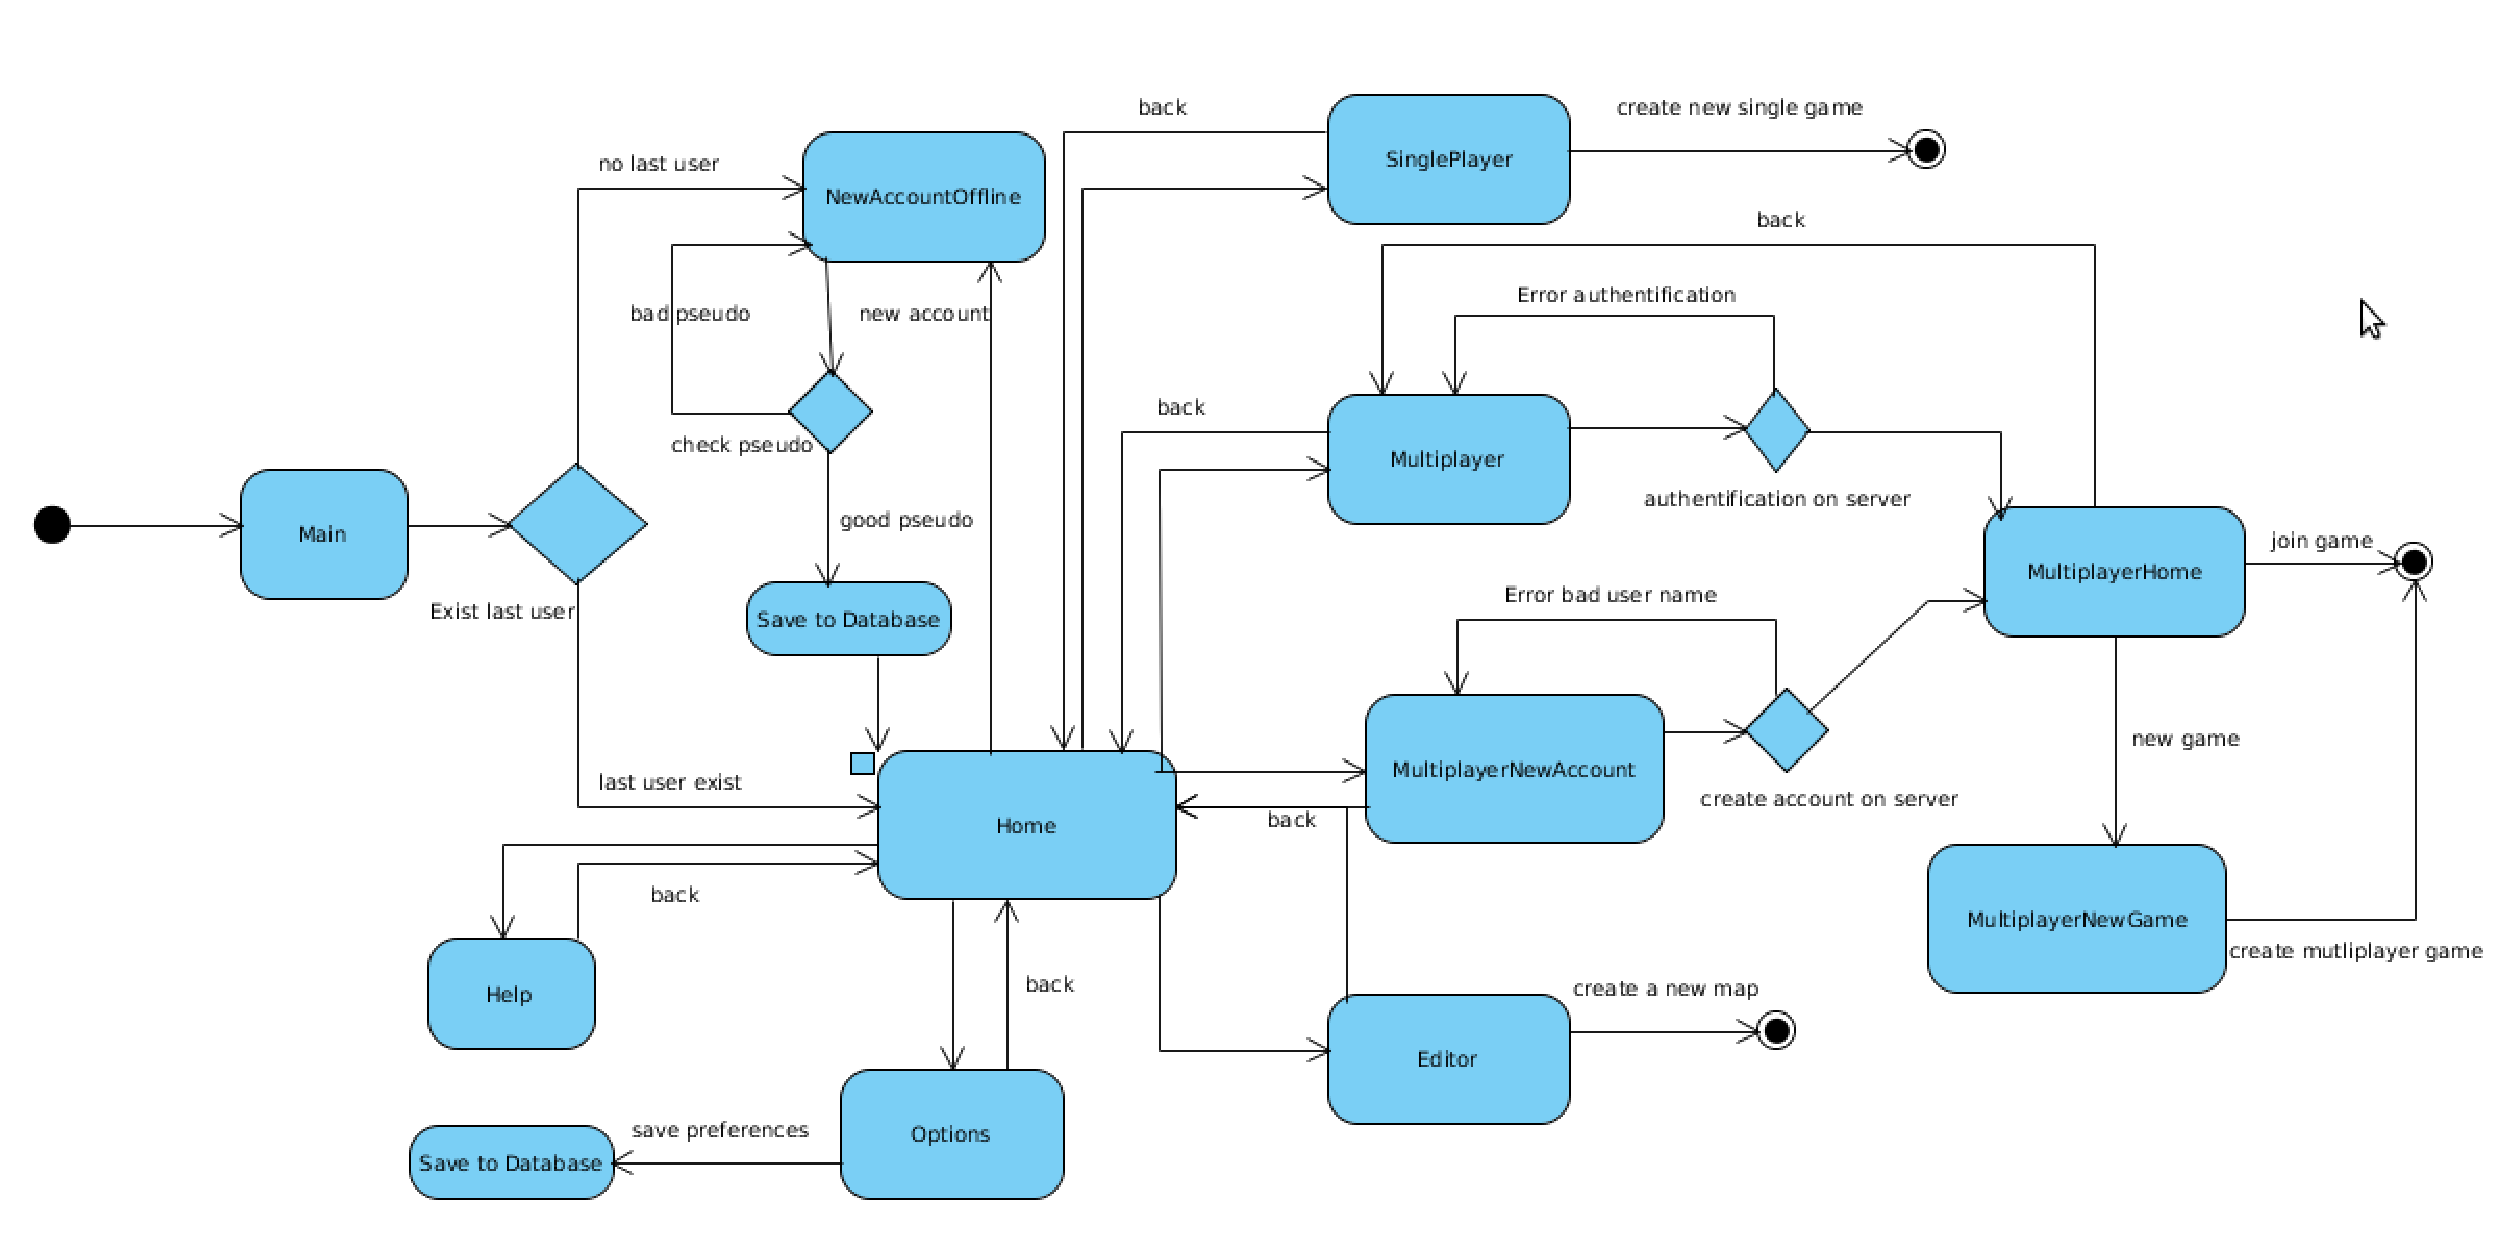
\includegraphics[width=23cm, angle=90]{./diagrammes/diag_activity.eps}
		\end{center}

				\paragraph{Base de données\\}
				
				Une base de données locale a elle aussi été conçue. Cette dernière a pour
				but de stocker plusieurs types de données.
				
				En effet dès lors qu'un compte local est crée sur le téléphone dans la
				table PlayerAccount, il est possible de conserver ses préférences de joueur
				tel que la couleur du joueur, le pseudonyme ou même ses paramètres de connexion multijoueur. 
				Vous pourrez créer autant de comptes locaux que vous le désirez, et il
				sera possible possible d'éditer ou choisir son compte.
				
				L'application est par ailleur en mesure de conserver
				les valeurs sonores, la langue et même le dernier utilisateur de
				l'application, grâce à un son id qui est clé étrangère dans la table System(lastUser).
				
				De plus l'application sera délivrée avec quelques cartes officielles, mais
				l'utilisateur aura libre droit de créer ses propres cartes de jeu via un
				éditeur. Elles seront alors stockées dans la table Map avec toujours une
				clé étrangère vers l'id de son créateur(owner). \\
				
				\begin{center}
				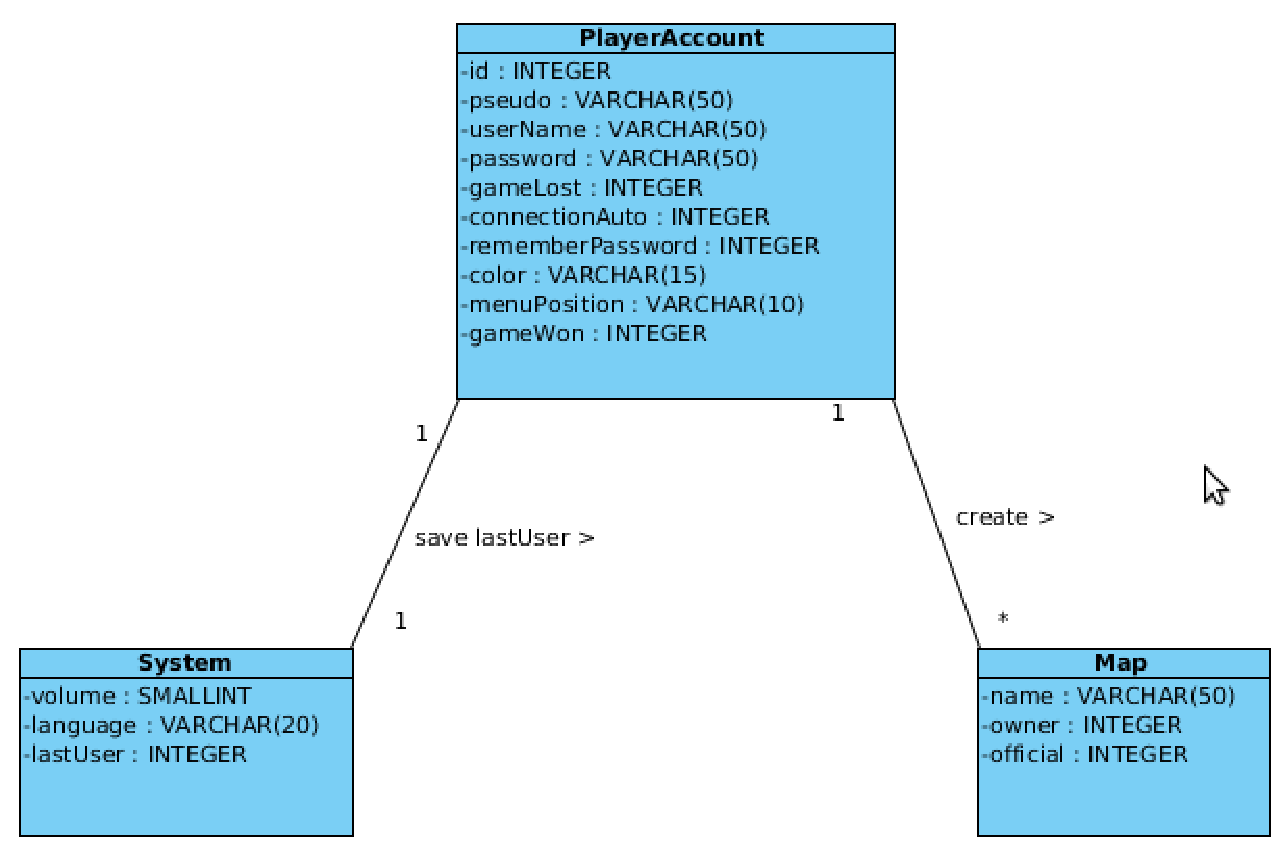
\includegraphics[width=11cm]{./diagrammes/menu_bdd.eps}
				\end{center}
				
				
				\paragraph{Scénarios}
			
		\subsection{Jeu}
			\begin{itemize}
				\item{Diagramme classe}
				\item{Gameplay}
				\item{Gestion images / tile mapping}
				\item{Images}
				\item{Sons}
			\end{itemize}
			
		\subsection{Réseau}
			\paragraph{Serveur\\}
			
			Il a été fixé dans le cahier des charges que notre serveur devrait pouvoir
			effectuer plusieurs tâches particulières séparées. Nous avons donc décidé de
			les compartimenter en classes.
			
			Les six éléments situés sur la partie haute du schéma
			ci-dessous(respectivement Inscription, Connection, GamesList, CreateGame,
			ConnectionGame et ManageGame), réprésente les différents tâches demandées.
			Elles sont reliées à une classe nommée contexte, qui leur permettra d'accéder
			aux mêmes données sans qu'il y ait de conflits. La partie basse représente les
			objets qui seront utilisés pour les parties en multijoueurs. Bien évidemment
			ces objets sont très proches de ceux utilisés dans les parties locales.
		
			\begin{center}
					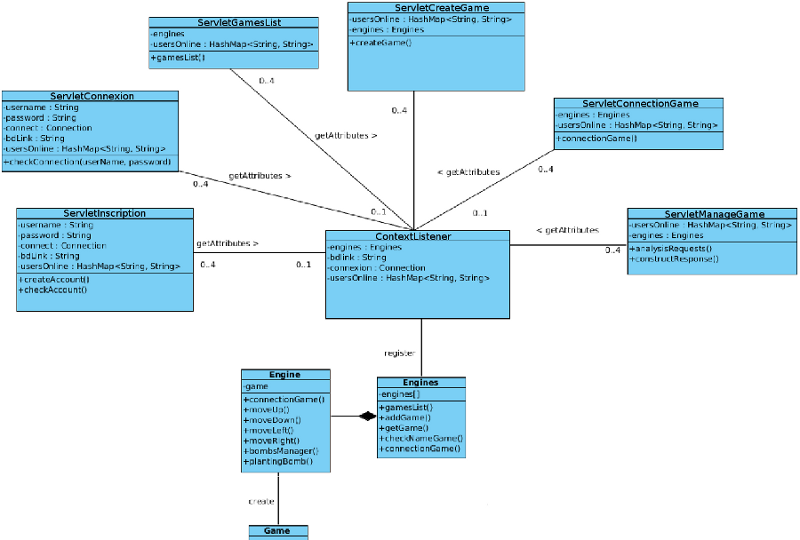
\includegraphics[scale = 0.5]{./diagrammes/serveur.eps}
			\end{center}
			
			
			\paragraph{Base de données\\}
			Afin de pouvoir conserver les utilisateurs en lignes ainsi que leurs infos
			personnels pour permettre une authentification, nous avons dû établir une
			base de données sur le serveur. Cette dernière à été pensé comme demandé pour 
			l'enregistrement de comptes. Une unique table nommée Users remplie donc cette
			fonction. Le serveur devra pouvoir y accéder en écriture(inscription) comme
			en lecture(connexion).
			
			Elle ne comportera que deux champs, userName et password.
						
	\section{Différences entre Android et iOS}
	


\chapter{Développement}
	\section{Mobile}
		\subsection{Menus}
			\subsubsection{API et widget}
			TODO ludo
		
		
			\subsubsection{BDD}
			Après avoir effectué divers recherches, il s'est avéré que le gestionnaire
			de bases de données utilisé sur les deux plateformes est SQLite 3. 
			
			\paragraph{Android\\}
			
			Pour manipuler aisément les bases de données depuis l'application,
			nous avons crée une classe héritant de \textit{SQLiteOpenHelper}. Cette
			dernière fournit des outils de manipulations. Un attribut y est
			instancié, il s'agit de la base de données elle même, de type
			\textit{SQLiteDatabase}.
			
			Nous y avons crée 3 Tables, \textit{PlayerAccount} sauvegardant toutes les
			informations sur les utilisateurs locaux, \textit{System} concervant les
			propriétés du système, et enfin \textit{Map} décrivant les informations
			relatives au cartes de jeu crées par l'utilisateur.
			
			Ainsi de nombreuses	fonctions ont été implémenté dans le but de simplifier les interactions
			avec cette base de données depuis l'application. Il est par exemple possible de créer un nouvel 
			utilisateur local, modifier ses préférences, gérer les configurations systèmes comme la langue ou le volume
			du son, ajoûter de nouvelles maps ou même récupérer toutes les informations
			concernant un utilisateur.\\
			
			Voici un exemple d'insertion d'un nouveau compte local dans la base de
			donnée. Rappelons que les tests d'existance du compte ont été fait depuis
			l'application même. Dans cet exemple vous verrez ainsi que nous commençons
			par récupérer les droits en écritures sur la base de données locale, puis
			nous créons un container qui servira à l'insertion de valeur dans la base. Et
			enfin l'insertion est faite. Nous terminons tout de même en fermant l'accès à
			cette base.
			
			Il s'agit la d'un schéma classique de fonction d'interaction avec notre
			base.
						
			\begin{verbatim}
			/** ajout compte hors ligne **/
				public long newAccount(String nomCompte){
					base = getWritableDatabase();
			
					ContentValues entree = new ContentValues();
					
					entree.put("pseudo", nomCompte);
					long var = base.insert("PlayerAccount", null, entree);
					
					base.close();
					return var;
				}
			\end{verbatim}

			
			\paragraph{iOS}
				
			\subsubsection{Première utilisation}
			\subsubsection{Création utilisateur}
			\subsubsection{Gestion utilisateur}
			\subsubsection{Gestion des préférences système}
			\subsubsection{Création de carte (charger)}
			\subsubsection{Création partie solo (tout)}
			\subsubsection{Création partie multi (officielle)}
			
		\subsection{Editeur de carte}
			\subsubsection{Rendu}
			\subsubsection{Interface utilisateur}
			\subsubsection{Sauvegarde}
		\subsection{Jeu}
			\subsubsection{Moteurs}
				\paragraph{Rendu}
					\subparagraph{Structure utilisée}
					\begin{itemize}
						\item{Pourquoi}
						\item{Avantages}
					\end{itemize}
				\paragraph{Physique}
					\subparagraph{Structure utilisée}
					\subparagraph{Mouvements (collisions)}
					\subparagraph{Gestion des bombes}
						\begin{itemize}
							\item{Threads}
						\end{itemize}
			\subsubsection{IA}
				\paragraph{Pathfinding}
					\subparagraph{A*}
					\subparagraph{Aléatoire}
				\paragraph{Prise de décision}
			\subsubsection{Interface utilisaeur}
				\paragraph{Android}
				\paragraph{iOS}
		
	\section{Serveur}
		Nous avons choisi de créer notre serveur sur une base de servlet. Ce fût ici
		aussi un point nouveau pour nous, réiterant les phases d'analyse, de
		découverte, de test et de mise en place. Le fonctionnement est basé sur les
		échanges de requêtes type HTTP, où à chaque demande correspond une réponse. 
		
		\subsection{Json}
		Soucieux des performances et de la rapidité des échanges entre applications et
		serveur, nous avons mis en place un protocole de communication client/serveur
		où les messages transitant sont des flux JSON. Ce dernier semblait être un
		format de données d'échanges optimal pour véhiculer le plus d'informations
		avec une taille moindre. De plus étant beaucoup utilisé, nos deux langages
		mettent à disposition des outils de sérialisation de leurs objets en JSON.
		
		\begin{verbatim}
		ServletInscription
			Player => Serveur
			{["username","password"]}
			
			Serveur => Player
			{"OK"} ou {"BU"}
			
		ServletConnexion 	
			Player => Serveur
			{["username","password"]}
			
			Serveur => Player
			{"OK"} ou {"BU"}
			
		ServletGameList
			Player => Serveur
			{"userKey"}
		
			Serveur => Player
			{[{"class":"Game","map":"mapName","name":"gameName",
			 "playerNumberConnected":nbConnected,"type":"gameType"},{..},{..}]}
			 
		ServletCreateGame:
			Player => Server:
				{"userKey": <userKey>, "game": {"name":<name>, "type":<type>, "map":<map>, "ennemiesNumber": <ennemiesNumber>}}
				
			Server => Player:
				{"OK"} ou {"errorType"}
			 
		ServletConnectionGame:
			Player => Server:
				{["userKey", "gameName"]}
				
			Server => Player:
				{[<1/2/3/4>, "play<true/false>", "map", "time<mm:ss>"]} 
				ou 
				{"errorType"}
				
		ServletManageGame:
			Player => Server: 
				{"userKey", "gameName", "action"}	
				
			Server => Players: (Player, bombs, blocs, score, time)
				{[
				 [ ["x", "y", "direction", "dead <true/false>"],[...] ],
				 [ ["x", "y", "type", "explode <true/false>" ], [...] ],
				 [ ["position": {"x", "y"}, "bonus": <bonus>], [..] ],
				 [1,2,3,4],
				 "time <mm:ss>"]} 
				 ou 
				{"errorType"}
			 
			 
		\end{verbatim}
		
		\subsection{Servlet}
		Comme il a été dit précédement, notre serveur est accessible via des requêtes
		HTTP contactant des servlets. Ces servlets sont stockées dans un serveur
		d'application nommé Apache Tomcat. Il s'agit d'un conteneur libre de
		servlets Java 2 Enterprise Edition, mais il fait aussi office de serveur
		Web.
		
		Une servlet est une classe Java qui permet de créer dynamiquement des données
		au sein d'un serveur HTTP. Une servlet s'exécute dynamiquement sur le serveur
		web et permet l'extension des fonctions de ce dernier, typiquement : accès à
		des bases de données.
		
		\subsubsection{Schéma de fonctionnement }
		
		\begin{center}
			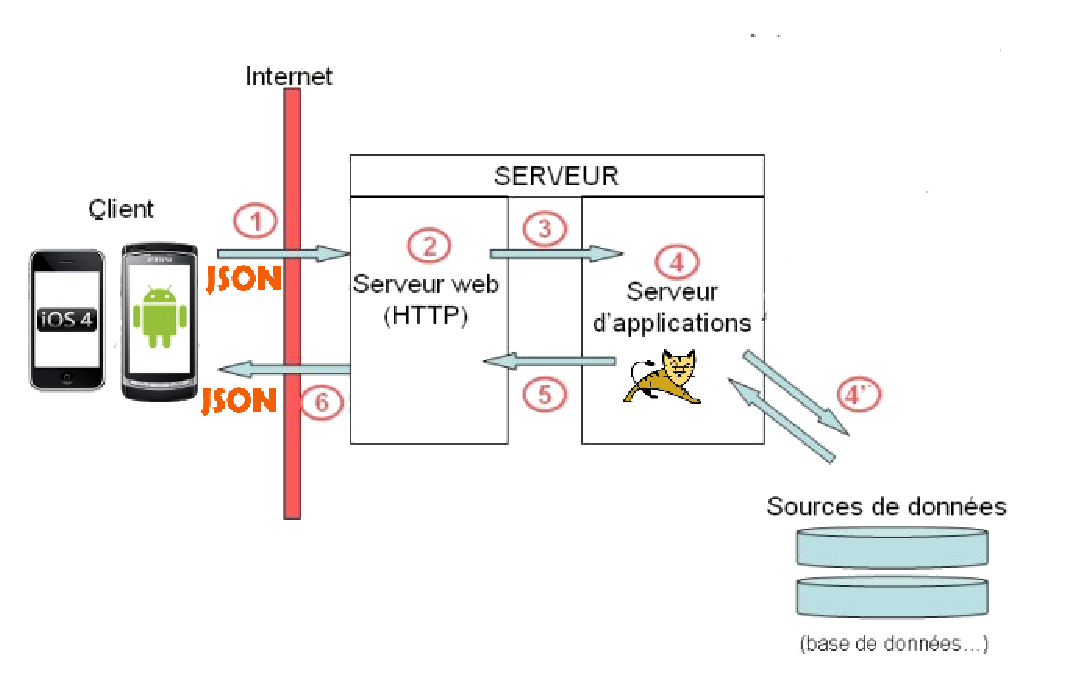
\includegraphics[width=16cm]{./diagrammes/serveurappli.eps}
		\end{center}
		
		\begin{enumerate}
		 \item Le client émet une requête pour demander une
			ressource au serveur. Par exemple la création de son compte multijoueur,
			qui pourrait se situer \url{http://Bomberklob.com/inscription}
		\item Côté serveur, c'est le serveur web qui traite les
			requêtes HTTP entrantes. Il traite donc toutes les requêtes, qu'elles
			demandent une ressource statique ou dynamique. Seulement, un serveur HTTP ne
			sait répondre qu'aux requêtes visant des ressources statiques.
		\item Ainsi, si le serveur HTTP s'aperçoit que la requête reçue est destinée
		au serveur d'applications, il la lui transmet. Les deux serveurs sont reliés par un canal, nommé connecteur.
		
		\item Le serveur d'applications (dans notre cas Tomcat) reçoit la requête à
		son tour. Lui est en mesure de la traiter. Il exécute donc la servlet
		correspondante à la requête, en fonction de l'URL, en récupérant les valeurs
		dans le flux JSON entrant. Cette opération est effectuée à partir de la
		configuration du serveur, grâce un fichier web.xml faisant le mapping entre URL et servlet associée. 
		
		La servlet est donc invoquée, et le serveur lui fournit notamment deux objets
		Java exploitables: un représentant la requête, l'autre représentant la réponse.
		La servlet execute sa fonction et génère la réponse à la demande, sous forme
		de flux JSON. Cela peut passer par la consultation de sources de données,
		comme des bases de données (4' sur le schéma).		
		
		\end{enumerate}
		
		
		\subsubsection{En pratique}
		
		Le requetes font appel à la fonction post des servlet. Le flux entrant étant
		de type JSON, il faut déserialiser le flux dans un objet correspondant. Exemple
		l'utilisateur envoie son userName et son mot de passe crypté dans un tableau,
		sérialisé en JSON, pour pouvoir récupérer les informations nous procédons
		comme suit: 
		
		\begin{verbatim}
			BufferedReader req = 
				  new BufferedReader(new InputStreamReader(request.getInputStream()));
			OutputStreamWriter writer = 
				  new OutputStreamWriter(response.getOutputStream());
			String message = req.readLine();
			
			if (message != null) {
				  response.setContentType("text/html");
				
				   // désérialisation des infos de l'utilisateur dans une arraylist 
				  JSONDeserializer<ArrayList<String>> jsonDeserializer = 
					  new JSONDeserializer<ArrayList<String>>();
				  ArrayList<String> identifiers;
				  identifiers = jsonDeserializer.deserialize(message);
				
				  username = identifiers.get(0);
				  password = identifiers.get(1);
				  
			  ...}
		\end{verbatim}
		
		
		\subsubsection{La sécurité}
		Ce serveur de jeu étant hebergé sur internet et contenant des informations
		sensibles d'utilisateurs, tels que des mots de passes, il était crucial
		d'instaurer des règles de sécurité et de cryptage. 
		
		En effet lors des inscriptions ou connexion au serveur pour le mode
		multijoueur, les mots de passes sont tout d'abord cryptés côté client et
		ensuite encapsulé dans un flux JSON, pour être envoyé au serveur. Il stockera
		ainsi la chaine de caractères extraite de l'objet déserialisé. De cette
		manière à aucun moment les données confidentielles ne transiteront en clair.
		
		De plus un mécanisme de session est en place. Dans la confirmation de
		connexion ou d'inscription, une userKey est générée. Elle correspond en
		réalité à l'identifiant de session envoyé par le serveur. Une fois associée
		à l'username correspondant, le tout est ajoûté dans le tableau d'utilisateurs
		connectés.
		Cet userKey est ensuite nécessaire pour contacter les servlets suivantes. Si
		cet identifiant n'est pas envoyé ou n'est pas présent dans le tableaux des
		utilisateurs connectés, il sera alors impossible d'accéder aux ressources du
		serveur.
		
		\subsection{BDD}
		La base de données du serveur n'est pas très complexe. En effet elle ne fait
		qu'accueillir les couples userName/password des utilisateurs dans la
		table Users. 
		Pour son accès, chaque servlet peut récupérer un objet de type Connection,
		instancié à l'initialisation du serveur. Il permettra à son tour
		de récuperer un objet de type Statement. L'application va l'employer pour
		transmettre des instructions à la base. Exemple d'insertion: 
		
		\begin{verbatim}
		Statement theStatement = connection.createStatement();
		theStatement.execute(
		     "INSERT into Users VALUES ('"+ username +"','"+password+"')");
		\end{verbatim}
		
		
		
		
\chapter{Manuel d'utilisation}
	\section{Menus}
	TODO ludo
	\section{Jeu}
	\section{Editeur}
	

\chapter{Discussion}
	\section{Problèmes}
		\subsection{Android}
		\subsection{iOS}
	\section{Améliorations}
		\subsection{Jeu}
		\subsection{Serveur}
			\begin{itemize}
				\item{Pooling}
				\item{Session}
			\end{itemize}
			
\chapter{Conclusion}

\end{document}
